\section{}
Determine whether the following stress distribution is a valid solution for a two-dimensional problem:
\begin{equation*}
    \sigma_x = -ax^2y, \quad \sigma_y = -\frac{1}{3}ay^3, \quad \tau_{xy} = -axy^2
\end{equation*}
where $a$ is a constant. Body forces may be neglected.

% \begin{figure}[h]
%     \centering
%     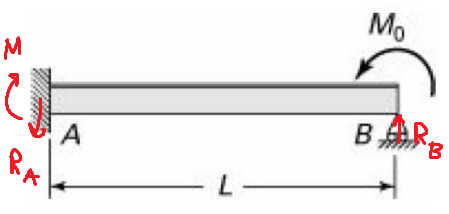
\includegraphics[width=0.5\linewidth]{Questions/Figures/Q2ProblemDiagram.png}
%     \caption{Two-dimensional plane stress problem.}
%     \label{fig:Q2ProblemDiagram}
% \end{figure}

The compatibility equation is
\begin{equation*}
    \nabla^4 \Phi = \frac{\partial^4 \Phi}{\partial x^4} + 2 \frac{\partial^4 \Phi}{\partial x^2 \partial y^2} + \frac{\partial^4 \Phi}{\partial y^4} = 0
\end{equation*}
Term by term,
\begin{align*}
    \frac{\partial^4 \Phi}{\partial x^4} &= \frac{\partial^2}{\partial x^2} \sigma_y \\
    &= \frac{\partial^2}{\partial x^2} \left( -\frac{1}{3}ay^3 \right) \\
    &= 0 \\
    \frac{\partial^4 \Phi}{\partial y^4} &= \frac{\partial^2}{\partial y^2} \sigma_x \\
    &= \frac{\partial^2}{\partial y^2} \left( -ax^2y \right) \\
    &= 0 \\
    \frac{\partial^4 \Phi}{\partial x^2 \partial y^2} &= \frac{\partial^2}{\partial x^2} \sigma_x \\
    &= \frac{\partial^2}{\partial x^2} \left( -ax^2y \right) \\
    &= -2ay
\end{align*}
Therefore,
\begin{align*}
    \nabla^4 \Phi &= \frac{\partial^4 \Phi}{\partial x^4} + 2 \frac{\partial^4 \Phi}{\partial x^2 \partial y^2} + \frac{\partial^4 \Phi}{\partial y^4} \\
    &= 0 + 2(-2ay) + 0 \\
    &= -4ay
\end{align*}
Since $\nabla^4 \Phi \neq 0$, the stress distribution is \textbf{not} a valid solution for a two-dimensional problem.